\chapter{天体辐射机制的量子语言}
\label{chap:09}

\begin{chapteropening}
同一个平均谱可以来自不同的光场。热辐射、自由自由辐射、同步辐射、逆康普顿散射、maser 和曲率辐射都能写出 \(I_\nu\)，但它们在相干时间、偏振、亮温、光子聚束和跨频相关上并不相同。把辐射机制写成光子统计问题后，谱指数和光变曲线会自然扩展为 \(g^{(2)}(\tau)\)、偏振分辨相关、频率通道之间的联合概率和事件到达时间分布 \citep{1963PhRv..130.2529G,1963PhRv..131.2766G,1995ocqo.book.....M,1956Natur.177...27B,2017MNRAS.472.4126G}。
\end{chapteropening}

\section{为什么平均谱不够}

辐射机制的传统入口是比强度 \(I_\nu\)，也就是单位时间、单位面积、单位频率、单位立体角内的辐射能流。若源在天空上的立体角为 \(\Omega_{\rm s}\)，观测到的流量密度近似为 \(S_\nu\simeq I_\nu\Omega_{\rm s}\)。在射电和远红外常用 Rayleigh--Jeans 形式定义亮温
\begin{equation}
  T_b=\frac{c^2 I_\nu}{2k_B\nu^2}
      =\frac{c^2 S_\nu}{2k_B\nu^2\Omega_{\rm s}} .
  \label{eq:ch09-brightness-temperature}
\end{equation}
\begin{formulaexplain}
\(T_b\) 是亮温；\(I_\nu\) 是比强度，\(S_\nu\) 是流量密度，\(\Omega_{\rm s}\) 是源立体角。它把平均辐射强度换算成 Rayleigh--Jeans 等效温度，用来判断是否需要非热或相干机制。
\end{formulaexplain}
这里 \(c\) 是光速，\(k_B\) 是 Boltzmann 常数，\(\nu\) 是频率。\(T_b\) 的单位是 K。它等于“若辐射在 Rayleigh--Jeans 极限下来自黑体，需要什么温度才能给出同样 \(I_\nu\)”；对于非热粒子、maser 或 FRB，它不是物质热温度。用角直径估计 \(\Omega_{\rm s}\) 时，源越小，推得的 \(T_b\) 越高，因此时间尺度、VLBI 角尺寸和散射展宽都会直接进入辐射机制判断。

亮温把平均强度和源尺度接起来。Dulk 对太阳和恒星射电辐射的综述给出一个实用判据：非相干射电辐射的 \(T_b\) 通常难以超过 \(10^9\) 到 \(10^{10}~{\rm K}\)；显著高于这个范围的爆发需要相干机制，例如 plasma radiation 或 cyclotron maser \citep{1985ARA&A..23..169D}。FRB 更极端。一个毫秒、Jy 量级、Gpc 距离的射电脉冲给出
\begin{equation}
  T_b\simeq
  1.1\times10^{35}~{\rm K}
  \left(\frac{S_\nu}{1~{\rm Jy}}\right)
  \left(\frac{D_A}{1~{\rm Gpc}}\right)^2
  \left(\frac{t_{\rm FRB}}{1~{\rm ms}}\right)^{-2}
  \left(\frac{\nu}{1~{\rm GHz}}\right)^{-2},
  \label{eq:ch09-frb-tb}
\end{equation}
\begin{formulaexplain}
\(S_\nu\) 是脉冲流量密度，\(D_A\) 是角直径距离，\(t_{\rm FRB}\) 是宽度，\(\nu\) 是观测频率。这个估算说明毫秒尺度 FRB 的亮温远超非相干辐射上限。
\end{formulaexplain}
其中 \(D_A\) 是角直径距离，\(t_{\rm FRB}\) 是脉冲宽度。这个数量级远高于非相干粒子辐射上限，要求许多带电粒子在小于波长或相位可控的尺度上协同发射 \citep{2007Sci...318..777L,2018MNRAS.477.2470L,2019A&ARv..27....4P,2022A&ARv..30....2P}。

\begin{figure}[tbp]
\centering
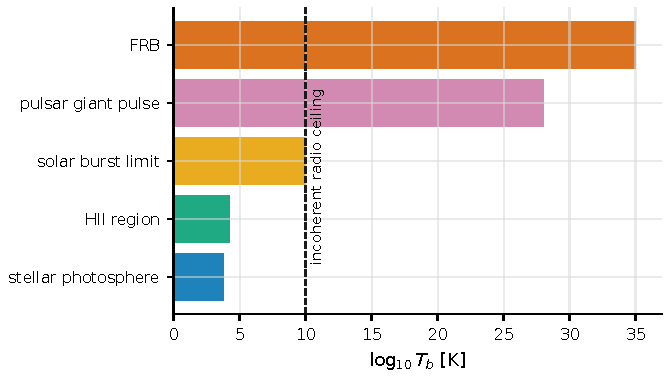
\includegraphics[width=0.82\linewidth]{figures/generated/chapter_09/ch09_brightness_temperature_scale.pdf}
\caption{亮温作为辐射机制判据。恒星光球和 HII 区处在普通热温度范围；太阳和恒星射电爆发若超过 \(10^{10}~{\rm K}\) 往往需要相干机制；脉冲星巨脉冲和 FRB 的亮温更高，只能由相干发射或强束射几何解释。虚线标出常用的非相干射电上限量级。}
\label{fig:chapter-09-brightness-temperature}
\end{figure}

亮温告诉我们“平均能量密度是否合理”，但不能告诉我们这些能量是由大量独立发射事件叠加出来的，还是由带电粒子协同发射出来的。两种光场可以有相同 \(I_\nu\)，却有不同的到达时间、偏振和跨频联合概率。平均谱之外，光子统计从一阶和二阶相干函数进入。若 \(E^{(+)}(t)\) 是正频电场算符，归一化一阶相干函数描述相位和频谱相干，
\begin{equation}
  g^{(1)}(\tau)=
  \frac{\langle E^{(-)}(t)E^{(+)}(t+\tau)\rangle}
       {\langle E^{(-)}(t)E^{(+)}(t)\rangle},
  \label{eq:ch09-g1}
\end{equation}
\begin{formulaexplain}
\(g^{(1)}(\tau)\) 是归一化一阶相干函数；\(E^{(+)}\) 和 \(E^{(-)}\) 是正、负频电场算符。它衡量场相位在时间延迟 \(\tau\) 后还保留多少记忆。
\end{formulaexplain}
而二阶相干函数描述强度涨落和光子到达时间相关，
\begin{equation}
  g^{(2)}(\tau)=
  \frac{\langle I(t)I(t+\tau)\rangle}{\langle I(t)\rangle^2}.
  \label{eq:ch09-g2}
\end{equation}
\begin{formulaexplain}
\(g^{(2)}(\tau)\) 是归一化强度相关；\(I(t)\) 是瞬时强度。它比较一个时刻的光子到达是否会提高另一个时刻的到达概率，是区分聚束、Poisson 和反聚束统计的核心量。
\end{formulaexplain}
式 \eqref{eq:ch09-g1} 问的是场本身隔多久还保留相位记忆，式 \eqref{eq:ch09-g2} 问的是一次光子到达是否会提高另一时刻光子到达的概率。热混沌光在单一时空偏振模式中有 \(g^{(2)}(0)=2\)，相干态有 \(g^{(2)}(0)=1\)。真实天文观测通常同时平均许多时间、频率、空间和偏振模式，热光聚束峰会被稀释为
\begin{equation}
  g^{(2)}_{\rm meas}(0)-1\simeq \frac{1}{M_{\rm eff}},
  \qquad
  M_{\rm eff}\simeq M_{\rm sp}M_{\rm pol}
  \left(1+\frac{\Delta t}{\tau_c}\right).
  \label{eq:ch09-mode-dilution}
\end{equation}
\begin{formulaexplain}
\(M_{\rm eff}\) 是有效混合模式数；\(M_{\rm sp}\)、\(M_{\rm pol}\) 分别是空间和偏振模式数，\(\Delta t/\tau_c\) 描述时间 bin 对相干时间的平均。模式越多，热光聚束对比度越低。
\end{formulaexplain}
\(M_{\rm sp}\) 是被混合的空间模式数，\(M_{\rm pol}\) 是偏振模式数，\(\Delta t\) 是电子或软件时间 bin，\(\tau_c\sim1/\Delta\nu\) 是由光谱带宽决定的相干时间。若 \(\Delta\nu=1~{\rm nm}\) 且 \(\lambda=500~{\rm nm}\)，\(\tau_c\sim0.8~{\rm ps}\)；若电子时间分辨率是 \(100~{\rm ps}\)，单模热光的聚束峰也会被压低两个数量级以上。窄带滤波、偏振选择和空间模式控制提高可见对比度，但会减少光子率。

\begin{figure}[tbp]
\centering
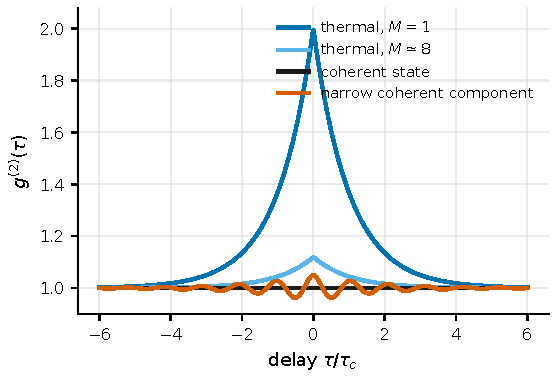
\includegraphics[width=0.82\linewidth]{figures/generated/chapter_09/ch09_radiation_g2_diagnostics.pdf}
\caption{不同光场的 \(g^{(2)}(\tau)\)。单模热光在零延迟处给出高度为 2 的聚束峰；多模平均把峰值压低；理想相干态接近 1；窄相干谱线或受激成分可以在接近 Poisson 的背景上留下小幅振荡或窄峰。横轴按相干时间 \(\tau_c\) 归一化。}
\label{fig:chapter-09-g2-diagnostics}
\end{figure}

\begin{figure}[tbp]
\centering
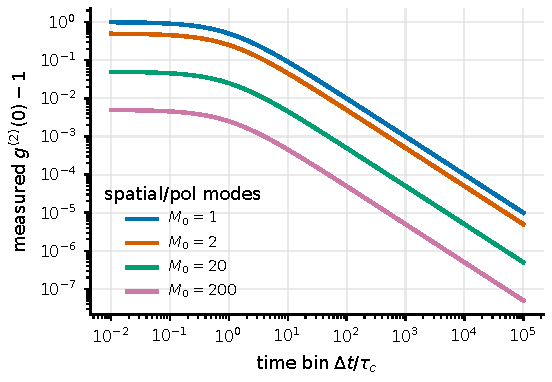
\includegraphics[width=0.82\linewidth]{figures/generated/chapter_09/ch09_thermal_mode_dilution.pdf}
\caption{热光聚束对比度随有效模式数下降。横轴是时间 bin 与相干时间的比值，曲线中的 \(M_0\) 代表进入同一个相关估计器的空间和偏振模式数。即使源本身是热光，宽时间 bin、多偏振混合或多空间模式混合都会让 \(g^{(2)}(0)-1\) 接近零。}
\label{fig:chapter-09-mode-dilution}
\end{figure}

\section{热过程怎样产生近似混沌光}

局部热平衡中的黑体光场由平均占有数
\begin{equation}
  \bar{n}_\nu=
  \frac{1}{\exp(h\nu/k_BT)-1}
  \label{eq:ch09-planck-occupation}
\end{equation}
\begin{formulaexplain}
\(\bar n_\nu\) 是频率 \(\nu\) 模式的平均光子占有数；\(h\nu\) 是单光子能量，\(T\) 是温度。Planck 分布给出热态每个模式中平均有多少光子。
\end{formulaexplain}
决定。这里 \(h\nu\) 是单光子能量，\(T\) 是物质温度。光球、尘埃和 CMB 接近这种热态；恒星光球的可见光 \(h\nu/k_BT\) 不一定处在 Rayleigh--Jeans 极限，因此颜色温度、有效温度和亮温不能混用。热光的相位由许多独立发射体随机叠加，电场近似复高斯过程；在这个条件下 Siegert 关系给出 \(g^{(2)}(\tau)=1+|g^{(1)}(\tau)|^2/M_{\rm eff}\)。

自由自由辐射不是黑体谱本身，而是许多电子在离子库仑场中被加速时发出的连续谱。关键物理图像仍然是“许多独立事件相加”：单次碰撞的相位不可预测，窄带内的复电场会趋向高斯随机过程。稀薄电离气体中，发射系数的数量级可写成
\begin{equation}
  j_\nu^{\rm ff}\propto
  n_e n_i T_e^{-1/2}
  \exp\!\left(-\frac{h\nu}{k_BT_e}\right)
  g_{\rm ff}(\nu,T_e),
  \label{eq:ch09-free-free}
\end{equation}
\begin{formulaexplain}
\(j_\nu^{\rm ff}\) 是自由自由发射系数；\(n_e,n_i\) 是电子和离子密度，\(T_e\) 是电子温度，\(g_{\rm ff}\) 是 Gaunt 因子。它描述许多独立库仑碰撞贡献的连续谱强度。
\end{formulaexplain}
其中 \(n_e\) 和 \(n_i\) 是电子和离子数密度，单位 \({\rm cm^{-3}}\) 或 \({\rm m^{-3}}\)；\(T_e\) 是电子温度；\(g_{\rm ff}\) 是 Gaunt 因子，通常为 1 到数十量级。HII 区的 \(T_e\sim10^4~{\rm K}\)，星风和吸积流可以更高。许多独立碰撞事件叠加后，光场在窄带内仍接近混沌热光；但若观测时间远大于 \(\tau_c\)，可见聚束会被式 \eqref{eq:ch09-mode-dilution} 稀释。

吸收和发射要放在辐射转移方程里：
\begin{equation}
  \frac{{\rm d}I_\nu}{{\rm d}s}=j_\nu-\alpha_\nu I_\nu,
  \qquad
  S_\nu=\frac{j_\nu}{\alpha_\nu}.
  \label{eq:ch09-radiative-transfer}
\end{equation}
\begin{formulaexplain}
\({\rm d}I_\nu/{\rm d}s\) 是视线方向上的强度变化；\(j_\nu\) 加入辐射，\(\alpha_\nu I_\nu\) 吸收辐射，\(S_\nu\) 是源函数。辐射转移把发射机制和光深效应连在一起。
\end{formulaexplain}
\(s\) 是沿视线距离，\(j_\nu\) 是发射系数，\(\alpha_\nu\) 是吸收系数，\(S_\nu\) 是源函数。若换成亮温并用光深 \({\rm d}\tau_\nu=\alpha_\nu{\rm d}s\)，均匀 slab 给出
\begin{equation}
  T_b=T_{\rm eff}\left(1-e^{-\tau_\nu}\right)
      +T_{\rm bg}e^{-\tau_\nu}.
  \label{eq:ch09-tb-transfer}
\end{equation}
\begin{formulaexplain}
\(T_b\) 是出射亮温；\(T_{\rm eff}\) 是源函数对应温度，\(T_{\rm bg}\) 是背景亮温，\(\tau_\nu\) 是光深。薄源只贡献小增量，厚源趋向自身源函数。
\end{formulaexplain}
\(T_{\rm eff}\) 是对应源函数的等效温度，\(T_{\rm bg}\) 是背景亮温。光深很小时 \(T_b\simeq T_{\rm eff}\tau_\nu+T_{\rm bg}\)，光深很大时 \(T_b\to T_{\rm eff}\)。这条式子常用于判断一个源是热化、半透明还是非热发射占优 \citep{1979rpa..book.....R,2011piim.book.....D,1985ARA&A..23..169D}。

\section{非热粒子怎样改变谱和偏振}

同步辐射来自相对论电子在磁场中的螺旋运动。单个电子的特征频率为
\begin{equation}
  \nu_c=\frac{3eB\sin\alpha}{4\pi m_ec}\gamma^2 ,
  \label{eq:ch09-synch-critical}
\end{equation}
\begin{formulaexplain}
\(\nu_c\) 是同步辐射特征频率；\(B\) 是磁场，\(\alpha\) 是 pitch angle，\(\gamma\) 是电子 Lorentz 因子。频率随 \(B\) 和 \(\gamma^2\) 增长，所以高能电子可把辐射推到高频。
\end{formulaexplain}
其中 \(e\) 是元电荷，\(B\) 是磁场强度，\(\alpha\) 是 pitch angle，\(m_e\) 是电子质量，\(\gamma\) 是 Lorentz 因子。若 \(B=1~{\rm G}\)、\(\gamma=10^3\)、\(\sin\alpha=1\)，则 \(\nu_c\simeq4.2\times10^{12}~{\rm Hz}\)，在远红外。若 \(B=10^{-5}~{\rm G}\) 的星系际或喷流尺度磁场中，同样电子主要辐射射电。单电子功率的能谱很宽，真实源的发射系数来自
\begin{equation}
  j_\nu^{\rm syn}=\int P_\nu(E,B,\alpha)\,N(E)\,{\rm d}E .
  \label{eq:ch09-synch-emissivity}
\end{equation}
\begin{formulaexplain}
\(j_\nu^{\rm syn}\) 是同步辐射发射系数；\(P_\nu\) 是单电子功率谱，\(N(E)\) 是电子能量分布。积分表示观测谱是所有能量电子贡献的叠加。
\end{formulaexplain}
\Needspace{12\baselineskip}
若电子能谱 \(N(E)\propto E^{-p}\)，光薄同步辐射给出 \(I_\nu\propto\nu^{-\alpha_{\rm syn}}\)，其中 \(\alpha_{\rm syn}=(p-1)/2\)。最大线偏振度在均匀磁场中约为
\begin{equation}
  \Pi_{\rm syn}=\frac{p+1}{p+7/3}.
  \label{eq:ch09-synch-polarization}
\end{equation}
\begin{formulaexplain}
\(\Pi_{\rm syn}\) 是光薄同步辐射的最大线偏振度；\(p\) 是电子能谱指数。它给出均匀磁场和幂律电子分布下偏振能达到的理论上限。
\end{formulaexplain}
例如 \(p=2.4\) 时 \(\Pi_{\rm syn}\simeq72\%\)。实际喷流、超新星遗迹和脉冲星风云的偏振往往较低，因为磁场方向、法拉第旋转、束内平均和多发射区叠加会抵消偏振。由大量独立电子和湍动单元叠加时，电场也可近似高斯混沌场；与热光不同的是，平均谱和偏振由非热粒子分布和磁场几何决定 \citep{1965ARA&A...3..297G,1970RvMP...42..237B,1978bllo.conf..328B,2012ApJ...752..157Z}。

逆康普顿散射把低能光子提升到高能。Thomson 极限中，散射后光子能量的数量级为
\begin{equation}
  h\nu_{\rm IC}\sim \gamma^2 h\nu_{\rm seed}.
  \label{eq:ch09-ic-energy}
\end{equation}
\begin{formulaexplain}
\(h\nu_{\rm seed}\) 是种子光子能量，\(h\nu_{\rm IC}\) 是散射后能量，\(\gamma\) 是电子 Lorentz 因子。逆康普顿散射在 Thomson 极限中把光子能量提升约 \(\gamma^2\) 倍。
\end{formulaexplain}
热电子云中的多次散射常用 Compton \(y\) 参数判断：
\begin{equation}
  y\simeq
  4\frac{k_BT_e}{m_ec^2}\max(\tau_T,\tau_T^2),
  \label{eq:ch09-compton-y}
\end{equation}
\begin{formulaexplain}
\(y\) 是 Comptonization 强度参数；前因子是单次散射的相对能量增益，\(\max(\tau_T,\tau_T^2)\) 估计平均散射次数。它判断谱会被电子云改写到什么程度。
\end{formulaexplain}
其中 \(T_e\) 是电子温度，\(\tau_T\) 是 Thomson 光深。\(y\ll1\) 时谱只被轻微改变；\(y\sim1\) 时会形成明显的 Comptonized continuum；\(y\gg1\) 时趋向饱和 Comptonization。X 射线双星、AGN corona 和 GRB photosphere 模型中，平均谱可以由同步、热光子和逆康普顿多分量混合形成，单靠谱指数很难唯一判定机制 \citep{1980A&A....86..121S,1999MNRAS.309..496G,2013ApJ...765..103L}。

\begin{figure}[tbp]
\centering
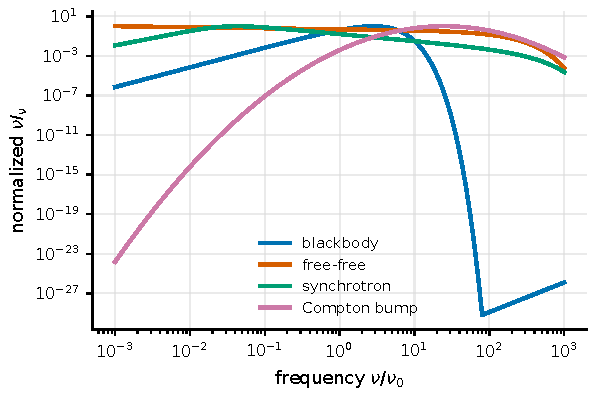
\includegraphics[width=0.84\linewidth]{figures/generated/chapter_09/ch09_spectral_mechanisms.pdf}
\caption{常见连续辐射机制的归一化谱形示意。黑体有热峰和 Rayleigh--Jeans 低频端；自由自由辐射在射电可近似平坦并在高频指数衰减；同步辐射由非热电子能谱给出幂律和高低频截断；逆康普顿分量常表现为高能 bump。真实源需要把这些分量放进辐射转移和几何模型中联合拟合。}
\label{fig:chapter-09-spectral-mechanisms}
\end{figure}

\section{相干机制怎样突破亮温上限}

Maser 从负吸收开始。若某条谱线存在粒子数反转，吸收系数可为负，写成 \(\alpha_\nu<0\)。沿路径的强度近似满足
\begin{equation}
  I_\nu(L)\simeq I_\nu(0)\exp(|\tau_m|),
  \qquad
  \tau_m=\int_0^L\alpha_\nu\,{\rm d}s<0 .
  \label{eq:ch09-maser-gain}
\end{equation}
\begin{formulaexplain}
\(I_\nu(0)\) 和 \(I_\nu(L)\) 是路径前后的强度；\(\tau_m<0\) 是负吸收光深。Maser 的无饱和增益随 \(|\tau_m|\) 指数增长，这是高亮温窄线的来源。
\end{formulaexplain}
无饱和时，增益对光深指数敏感；饱和后，受激辐射耗尽反转，线宽、偏振和强度随泵浦与几何改变。水 maser、OH maser 和 SiO maser 的亮温可极高，但它们的相干性通常由许多速度相干路径、湍动团块和偏振传播效应共同决定，不能简单等同于实验室单模激光。Goldreich、Keeley、Kwan 和 Elitzur 的工作给出了源尺寸、饱和、线宽与偏振的基本约束 \citep{1972ApJ...174..517G,1973ApJ...179..111G,1974ApJ...190...27G,1982RvMP...54.1225E,1992ARA&A..30...75E}。

电子回旋 maser 是强磁化低密度等离子体中的相干射电机制。它要求电子分布偏离平衡，例如 loss-cone 分布，并且磁场频率与等离子体频率的关系允许电磁波逃逸。回旋频率为
\begin{equation}
  \nu_B=\frac{eB}{2\pi m_ec}
       \simeq 2.8~{\rm MHz}\left(\frac{B}{1~{\rm G}}\right).
  \label{eq:ch09-cyclotron-frequency}
\end{equation}
\begin{formulaexplain}
\(\nu_B\) 是电子回旋频率；\(e\) 是电荷，\(B\) 是磁场，\(m_e\) 是电子质量。观测到的 maser 频率可反推发射区磁场量级。
\end{formulaexplain}
若在 GHz 频率看到基频或低次谐波 electron-cyclotron maser，磁场量级是几百 G 到几 kG。太阳、行星、褐矮星和低质量恒星的高圆偏振射电爆发都可落在这个框架中 \citep{1982ApJ...259..844M,2006A&ARv..13..229T,2008ApJ...684..644H,1985ARA&A..23..169D}。

曲率辐射展示了另一条通往相干性的路。它不一定依赖能级反转，而是让许多电荷在相位上协同运动。相对论电荷沿弯曲磁力线运动时，单个电荷的特征频率和功率为
\begin{equation}
  \nu_{\rm curv}=\frac{3c}{4\pi\rho}\gamma^3,
  \qquad
  P_{\rm curv}=\frac{2e^2c}{3\rho^2}\gamma^4 ,
  \label{eq:ch09-curvature}
\end{equation}
\begin{formulaexplain}
\(\nu_{\rm curv}\) 是曲率辐射特征频率，\(P_{\rm curv}\) 是单粒子功率；\(\rho\) 是磁力线曲率半径，\(\gamma\) 是 Lorentz 因子。相干曲率辐射还需要许多电荷相位同步。
\end{formulaexplain}
其中 \(\rho\) 是磁力线曲率半径。若 \(\rho=10^7~{\rm cm}\) 且 \(\gamma=300\)，\(\nu_{\rm curv}\sim2\times10^9~{\rm Hz}\)。单个粒子的曲率辐射仍然太弱；相干曲率辐射要求许多电荷在小于波长的纵向尺度上成团，电场振幅相加，功率可近似随粒子数平方增长。这个思路长期用于脉冲星相干射电，也被用于 FRB 模型 \citep{1977ApJ...212..800C,2018MNRAS.477.2470L}。

FRB 的观测把这些机制推到极端。Lorimer burst 给出了毫秒时间尺度、冷等离子体色散和 \(T_b\sim10^{34}~{\rm K}\) 量级的第一组证据；重复源和 CHIME 样本显示，重复、偏振、漂移、微结构和宿主环境都会进入模型；SGR 1935+2154 的 2020 年事件把银河系 magnetar 和 FRB-like radio burst 直接连在一起 \citep{2007Sci...318..777L,2019A&ARv..27....4P,2022A&ARv..30....2P,2020Natur.587...54C,2020Natur.587...59B}。许多模型可分成两类：靠 population inversion 或激波产生的 maser 类机制，以及靠电荷团块或电流片产生的 antenna/curvature 类机制。微秒以下结构、强偏振、频率漂移和多波段非探测共同限制发射半径、Lorentz 因子、等离子体密度和辐射效率。

光学自然激光是另一种受激辐射案例。Eta Carinae 的 Weigelt blobs 中，Fe II 和 O I 线可在特定泵浦和光深条件下出现激光或激光样放大；这类线的宽度、空间位置、偏振和光子相关可检验反转与反馈几何 \citep{2004A&A...428..497J,2005NewA...10..361J,2008AIPC..984..216D}。受激辐射可以出现在射电 maser 之外的环境中；只要泵浦、能级结构和逃逸路径合适，光学谱线也可能带有非普通热光的统计特征。

\section{怎样把机制判断变成联合诊断}

实际分类时，平均谱只给第一层线索。区分热源、同步源、maser 和相干爆发，需要把谱、偏振、相关函数、时间尺度和角尺度放在同一个观测向量里：
\begin{equation}
  {\bf d}=
  \left\{
  I_\nu(t),\,
  Q_\nu(t),U_\nu(t),V_\nu(t),\,
  g^{(2)}_{ab}(\tau;\nu_i,\nu_j),\,
  \Delta t_{\rm var},\,
  \Omega_{\rm s}
  \right\}.
  \label{eq:ch09-diagnostic-vector}
\end{equation}
\begin{formulaexplain}
\({\bf d}\) 是机制诊断观测向量；它同时收集强度、Stokes 偏振、二阶相关、变异时间和角尺度。辐射机制判断需要这些量联合约束，而不是只看平均谱。
\end{formulaexplain}
\(Q,U,V\) 是 Stokes 参数，\(a,b\) 标记望远镜、偏振或频率通道，\(\Delta t_{\rm var}\) 是变异时间尺度，\(\Omega_{\rm s}\) 是角尺度约束。热源通常有低偏振、有限 \(T_b\) 和热聚束；光薄同步辐射可有高线偏振和幂律谱；maser 以窄线、高亮温和强偏振为特征；FRB 以极高亮温、毫秒到微秒结构、色散和强偏振为典型特征；散射和等离子体传播会改变时间结构和频谱，却不应被误认为源本身的发射统计。

\begin{figure}[tbp]
\centering
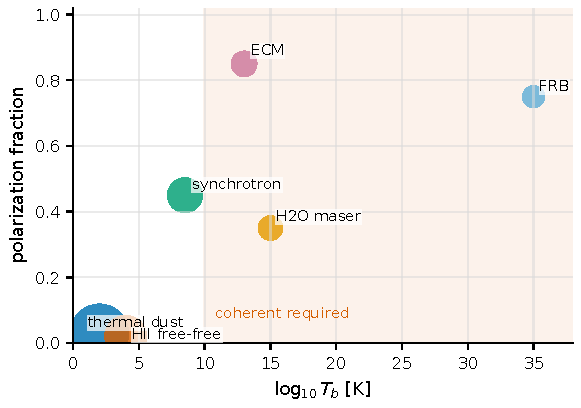
\includegraphics[width=0.86\linewidth]{figures/generated/chapter_09/ch09_diagnostic_plane.pdf}
\caption{辐射机制的联合诊断平面。横轴是亮温，纵轴是偏振分数，点大小表示可见二阶相干对比度的量级。热尘埃和 HII 区位于低亮温低偏振区域；同步辐射偏振较高但亮温通常低于相干爆发；electron-cyclotron maser、分子 maser 和 FRB 进入高亮温区域，需要解释相干发射、泵浦或电荷成团。}
\label{fig:chapter-09-diagnostic-plane}
\end{figure}

在数据分析中，\(g^{(2)}\) 的异常峰值要先和仪器、传播效应和混合源逐项比对。死时间、afterpulsing、时间戳量化和触发选择会改写到达时间相关；等离子体闪烁、散射尾、引力微透镜和频率依赖吸收会产生跨频相关；热背景叠加窄 maser 线，或同步连续谱叠加相干脉冲，也会让平均谱看起来平滑而光子统计不再单一。第 \ref{chap:06} 章和第 \ref{chap:07} 章的事件表、时间移位背景和协方差估计提供了这类排查所需的分析层。

